\documentclass[11pt,a4paper,oneside]{article}\usepackage[]{graphicx}\usepackage[]{color}
%% maxwidth is the original width if it is less than linewidth
%% otherwise use linewidth (to make sure the graphics do not exceed the margin)
\makeatletter
\def\maxwidth{ %
  \ifdim\Gin@nat@width>\linewidth
    \linewidth
  \else
    \Gin@nat@width
  \fi
}
\makeatother

\definecolor{fgcolor}{rgb}{0.345, 0.345, 0.345}
\newcommand{\hlnum}[1]{\textcolor[rgb]{0.686,0.059,0.569}{#1}}%
\newcommand{\hlstr}[1]{\textcolor[rgb]{0.192,0.494,0.8}{#1}}%
\newcommand{\hlcom}[1]{\textcolor[rgb]{0.678,0.584,0.686}{\textit{#1}}}%
\newcommand{\hlopt}[1]{\textcolor[rgb]{0,0,0}{#1}}%
\newcommand{\hlstd}[1]{\textcolor[rgb]{0.345,0.345,0.345}{#1}}%
\newcommand{\hlkwa}[1]{\textcolor[rgb]{0.161,0.373,0.58}{\textbf{#1}}}%
\newcommand{\hlkwb}[1]{\textcolor[rgb]{0.69,0.353,0.396}{#1}}%
\newcommand{\hlkwc}[1]{\textcolor[rgb]{0.333,0.667,0.333}{#1}}%
\newcommand{\hlkwd}[1]{\textcolor[rgb]{0.737,0.353,0.396}{\textbf{#1}}}%
\let\hlipl\hlkwb

\usepackage{framed}
\makeatletter
\newenvironment{kframe}{%
 \def\at@end@of@kframe{}%
 \ifinner\ifhmode%
  \def\at@end@of@kframe{\end{minipage}}%
  \begin{minipage}{\columnwidth}%
 \fi\fi%
 \def\FrameCommand##1{\hskip\@totalleftmargin \hskip-\fboxsep
 \colorbox{shadecolor}{##1}\hskip-\fboxsep
     % There is no \\@totalrightmargin, so:
     \hskip-\linewidth \hskip-\@totalleftmargin \hskip\columnwidth}%
 \MakeFramed {\advance\hsize-\width
   \@totalleftmargin\z@ \linewidth\hsize
   \@setminipage}}%
 {\par\unskip\endMakeFramed%
 \at@end@of@kframe}
\makeatother

\definecolor{shadecolor}{rgb}{.97, .97, .97}
\definecolor{messagecolor}{rgb}{0, 0, 0}
\definecolor{warningcolor}{rgb}{1, 0, 1}
\definecolor{errorcolor}{rgb}{1, 0, 0}
\newenvironment{knitrout}{}{} % an empty environment to be redefined in TeX

\usepackage{alltt}
\usepackage{amsmath,amsthm,amsfonts,amssymb}
\usepackage{pst-eucl,pstricks,pstricks-add,multido, pst-plot}
\usepackage[utf8]{inputenc}
%\usepackage[latin1]{inputenc}
\usepackage[spanish,activeacute]{babel}
\usepackage[a4paper,margin=2.5cm]{geometry}
\usepackage{times}
\usepackage[T1]{fontenc}
\usepackage{titlesec}
\usepackage{url}
\usepackage{float}
\usepackage{cite}
\usepackage{graphicx}
\usepackage{wrapfig}
\usepackage{lipsum}
\usepackage{multicol}
\usepackage{float}
\usepackage{lmodern}
\usepackage{epstopdf}
\parindent=0mm
\usepackage{color, colortbl}
\definecolor{azul}{rgb}{0.63, 0.79, 0.95}
\newtheorem{exm}{Example}[subsection]
\newtheorem{defi}[subsection]{Definition}
\newcommand*{\titleBOOK}{\begingroup
%\raggedleft
\centering
\vspace*{\baselineskip}
\vspace*{\baselineskip}
{\Huge\scshape Lecture Notes}\\[10mm]
%{\Large \includegraphics[scale=0.25]{uah.pdf}}\\[35mm]
{\Huge\scshape Non Life  \\[5mm]
Insurance} \\ [\baselineskip]
{\Large\bfseries First Draft}\\[0.3 \textheight]
{\Large Prof. Dr. Ricardo Gatto}\\
%{\large\scshape MS-PLUS, Inc.}\par
\vfill
\begin{center}
{\scshape Switzerland-Spain-Ecuador}\\
\rule{\textwidth}{0.5pt}
\end{center}
\vspace*{\baselineskip}
\endgroup}
\IfFileExists{upquote.sty}{\usepackage{upquote}}{}
\begin{document}
%\SweaveOpts{concordance=TRUE}
\titleBOOK
\newpage

\tableofcontents
\newpage


\section{Individual Risk and Distributions}
A non negative random variable is called a \textbf{loss} and it its distribution a \textbf{loss distribution}.\\
$X\sim Exponential(\alpha)$ means that $X$ has density $f_X(x)=\alpha e^{-\alpha x}$ and distribution function (d.f) $F_X(x)=1-e^{-\alpha x}$, $\forall x>0$ and $\alpha>0$.\\


Let $Y=e^x$, 
\begin{align*}
F_Y(Y) &= F_X(\log Y)\\
&=1-e^{\alpha \log (y)}\\
&=1-y^{-\alpha}
\end{align*}
Is called the \textbf{Pareto Distribution}. If $Y$ follows a Pareto distribution, denoted  $Y\sim Pareto(\alpha)$

\begin{knitrout}
\definecolor{shadecolor}{rgb}{0.969, 0.969, 0.969}\color{fgcolor}

{\centering 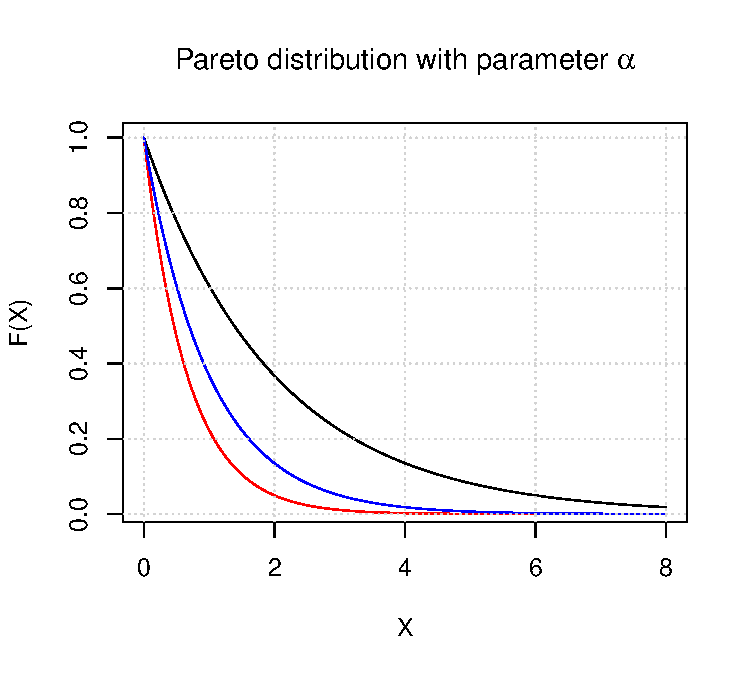
\includegraphics[width=\maxwidth]{figure/unnamed-chunk-1-1} 

}



\end{knitrout}

$X\sim Exponential (\lambda)$ and $Y\sim X^{\frac{1}{\tau}}$, $\forall \tau>0$
\begin{align*}
F_Y(Y) &= F_X(Y^{\tau})\\
&=1-e^{-\lambda y^{\tau}}, \quad \forall y>0\\
\end{align*}
$Y$ follows the \textbf{Weibull distribution}, $\tau$ is called the Weibull index.\\ It is denoted by $Y\sim Weibull(\tau,\lambda)$


\section{Thursday 09/03/17}

\subsection{Distribution of the largest claim amount}

The distribution of the largest loss is very important in \textbf{risk management}.

We will derive asymptotic aproximation of standardized maxima.

Let $X_1,\ldots,X_n$ be independent losses with distribution function (d.f) $F$ and define 
\[M_n=\max\{X_1,\ldots,X_n\}\]

\begin{align*}
P[M_n\leq n] &= P[X_1\leqx,..,X_n\leq x]\\
&=F^n(x), \quad  \forall x>0\\
\end{align*}

Let $\bar{x}=\sup\{x>0|F(x)<1\}$.

Assume $E[M_n]<\infty$, then $E[M_n]=\displaystyle\int_{0}^{\bar{x}}\{1-F^n(x)\}dx\xrightarrow{n\rightarrow \infty}{\bar{x}}$.

Assume $E[M^2_n]<\infty$, then $E[M_n^2]=\displaystyle\int_{0}^{\bar{x}}x\{1-F^n(x)\}dx\xrightarrow{n\rightarrow \infty}{\bar{x}^2}$

$Var(M_n)=E[M^2_n]-E^2[M_n]\xrightarrow{n\rightarrow \infty}{\bar{x}^2-\bar{x}^2}=0$, assuming $\bar{x}=0$.\newline

Thus the asymptotic distribution of $M_n$ is degenerate (the total mass is over $\bar{x}$). SO if we want to compute this asymptotic distribution, we must consider the standardization $\frac{M_n-b_n}{a_n}$.

Before studying these asymptotic approximation we give some examples with finite sample.
\subsection{Examples}
The distribution  of the monthly largest loss is Gumbel $F(x)=G(\frac{x-\mu}{\sigma})$ where $G(x)=exp\{-e^{-x}\}\ \ x\in\mathbb{R}$, what is the distribution of the annual maximum?
\begin{align*}
F^{12}&=\exp\{-12e^{-\frac{x-\mu}{\sigma}}\}\\
&=\exp\{-e^{-\frac{x-\mu}{\sigma}+log 12}\}\\
&=\exp\{-e^{-\frac{x-(\mu+\sigma log 12)}{\sigma}}\}
\end{align*}

It is thus agian Gumbel, with another location parameter with Frechet monthly largest loss, with $G(x)=\exp\{-x^{-\alpha}\}, \ x>0$, we have $F^{12}(x)=\exp\{-12\(\frac{x-\mu}{\sigma}\)^{-\alpha}\}=\exp\{-(\frac{x-\mu}{12^{\frac{1}{\alpha}}\sigma})^{-\alpha}\}$.
It is again Fréchet with another scale parameter. Because of this algebraic closure property, the Gumbel and the Frechet distributions are called max-stable.
We consider the slight generalization where the sample size is the random variable $N$.

Let $M_N=\max\{X_1,\ldots,X_N\}$. Assume $N$ independent of $X_1,X_2,\ldots$
\begin{align*}
P[M_N\leq x]&=\displaystyle\sum_{n=0}^{\infty}P[M_N\leq x|N=n]P[N=n]\\
&=\displaystyle\sum_{n=0}^{\infty}F^n(x)P[N=n]\\
&=G_N(F(x)), \quad \forall x\geq 0
\end{align*}

Where $M_0=0$ and $G_N(v)=\displaystyle\sum_{n=0}^{\infty}v^nP[N=n]$ is the generating function of $N$.

Thus $P[M_N\leq 0]$ if $F(0)=0$

\begin{exm}$N_k\sim Poisson(k,\lambda)$, the number of claim amounts during $k$ years.
\begin{align*}
G_{N_k}(v)&=E[v^{N_k}]\\
&=\displaystyle\sum_{n=0}^{\infty}v^ne^{-k\lambda}\frac{(k\lambda)^n}{n!}\\
&=e^{-k\lambda}\displaystyle\sum_{n=0}^{\infty}\frac{(\lambda kv)^n}{n!}\\
&=\exp\{-k\lambda+\lambda k v\}\\
&=\exp(\{k\lambda(v-1)\}\ \ \ \forall v\in\mathbb{R}\\
\end{align*}

Let $F(x)=1-e^{-\frac{x}{\sigma}}$
\begin{align*}
P[M_{N_k}\leq x]&=G_{N_k}(F(x))\\
&=\exp\{-k\lambda e^{-\frac{x}{\sigma}}\}\\
&=\exp\{-\exp\{-\frac{x}{\sigma+\log k\lambda}\}\}\\
&=\exp\{-\exp\{-\frac{x-\sigma \log  k\lambda}{\sigma}\}\}\\
\end{align*}
$\forall x\geq 0$ which is the Gumbel distribution.

Let $F(x)=1-(\frac{x}{\sigma}+1)^{-\alpha}\ \ \forall x\geq 0$
\begin{align*}
P[M_{N_k}\leq x]&=\exp\{k\lambda(\frac{x}{\sigma}+1)^{-\alpha}\}\\
&=\exp\{-(\frac{x}{\sigma(k\lambda)^{\frac{1}{\alpha}}}+1)^{-\alpha}\}\ \ \ \forall x \geq 0\\
\end{align*}

Which is the Fréchet distribution.
\end{exm}
\section{Pareto Type Distributions}
Extreme value theory is the analysis of the asymptotic distributions of standardized maxima.
We search for $a_1,a_2,...>0$, $b_1,b_2,....\in\mathbb{R}$ and for d.f $G$ s. t
$$P\left[\frac{M_n-b_n}{a_n}\leq x\right]\xrightarrow{n\rightarrow\infty}G(x)$$
at all continuity points $x\in\mathbb{R}$ of $G$

We consider distributions of Pareto-type.
\begin{defi}
The d.f F is of Pareto type if $$\lim_{x\rightarrow\infty}\frac{1-F(tx)}{1-F(x)}=t^{-\alpha}\ \ \forall t>0$$
for some $\alpha>0$
\end{defi}

\begin{exm}
F(x)=1-x^{-\alpha}\\
\frac{1-F(tx)}{1-F(x)}=\frac{(tx)^{-\alpha}}{x^{-\alpha}}=t^{\alpha}\ \ \forall x>1
\end{exm}


\begin{defi}
The function $f:\mathbb{R}_{+}\rightarrow \mathbb{R}_{+}$ has regular variation (to infinity) with index $\delta\in\mathbb{R}$,
$$\frac{f(tx)}{f(x)}\xrightarrow{x\rightarrow\infty}t^{\delta}$$
\end{defi}
This means that $f(tx)\sim t^{\delta}f(x)$, as $x\rightarrow\infty$ (Remember that a homogeneous function f of degree $\delta$ satisfies $f(tx)=t^{\delta}f(x)\ \ \forall x$).
 Notation $f\in\R_{\delta}$ Thus $F$ is of Pareto-type if and only if $1-F\in\mathbb{R}_{\alpha}$
 
 \begin{defi}
 The function $f:\mathbb{R}_+\rightarrow\mathbb{R}_+$ is a slow varying function if
 $$\frac{f(tx)}{f(x)}\xrightarrow{x\rightarrow\infty}1\ \ \forall t>0$$
 \end{defi}
 
 $f\in\mathbb{R}_{\delta}<=> f(x)=x^{\delta}l(x)$ where $l\in\mathbb{R}_0$\\
 =>
$$\frac{(tx)^{-\delta}f(tx)}{x^{-\delta}f(x)}=t^{-\delta}\frac{f(tx)}{f(x)}\xrightarrow{x\rightarrow\infty}t^{-\delta}t^{\delta}=1$$
  
  <=
 $$\frac{f(tx)}{f(x)}
  =\frac{(tx)^{\delta}l(tx)}{x^{\delta}l(x)}
 =t^{\delta}\frac{l(tx)}{l(x)}\xrightarrow{x\rightarrow\infty}t^{\delta}
$$

We want to show that if the distribution of the individual losses is of Pareto type, then the simple maxima is Fréchet distribution.

\begin{align*}
\log P\left[\frac{M_n-b_n}{a_n}\leq x\right] &= \log F^n(a_nx+b_n)\\
&=n\log F(a_nx+b_n)\\
&\sim\{1-F(a_nx+b_n)\}
\end{align*}
\begin{knitrout}
\definecolor{shadecolor}{rgb}{0.969, 0.969, 0.969}\color{fgcolor}

{\centering 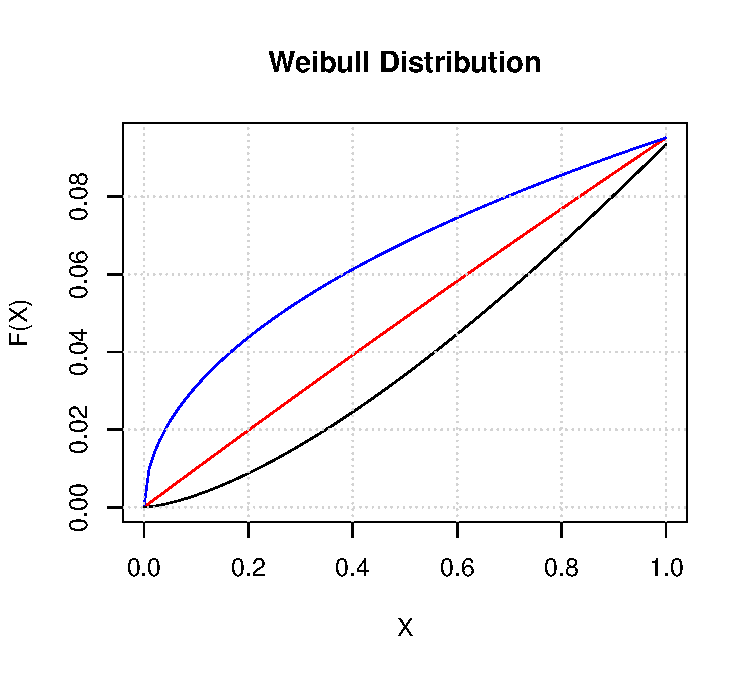
\includegraphics[width=\maxwidth]{figure/unnamed-chunk-2-1} 

}



\end{knitrout}

as $n\rightarrow \infty$, provided that $a_nx+b_n\xrightarrow{n\rightarrow\infty}\infty$ where
$a_1,a_2,...>0$ and $b_1,b_2,...\in\mathbb{R}$. Let us consider $F(x)=1-x^{-\alpha}\ \ \forall x \geq 1$ and $b_1=b_2=...=0$.

$$n\{1-F(a_nx)\}=n(a_nx)^{-\alpha}=x^{-\alpha}$$
would give us 
$$log P[\frac{M_n}{a_n}\leq x]\xrightarrow{n\rightarrow\infty}\exp\{-x^{-\alpha}\}$$
<=>
$$P[\frac{M_n}{a_n}\leq x]\xrightarrow{n\rightarrow\infty}\exp\{-x^{-\alpha}\}$$
$$\frac{M_n}{a_n}\xrightarrow{d} Fréchet(\alpha)$$
$$na_n^{-\alpha}=1<=>a_n^{-\alpha}=n^{-1}<=>a_n=n^{1/\alpha}$$
Thus $n^{1/\alpha}M_n\xrightarrow{d}Frechet(\alpha)$ as  can be expressed in terms of $F$ as follows.

$$1-x^{-\alpha}=u<=>x=(1-u)^{-1/\alpha}$$
$$F^{(-1)}(u)=(1-u)^{-1/\alpha}$$
$$F^{-1}(1-\frac{1}{n})=(1-\{1-\frac{1}{n}\})^{-\frac{1}{\alpha}}=(\frac{1}{n})^{-\frac{1}{\alpha}}$$
$$=n^{\frac{1}{\alpha}}=a_n$$

Thus $1-\frac{1}{n}=F(a_n)<=>$ $$\frac{1}{n}<=>1-F(a_n)<=>n=\{1-F(a_n)\}^{-1}$$

Let us keep this relation  for a more general distribution function $F$.

Thus
$$n\{1-F(a_nx)\}=\frac{1-F(a_nx)}{1-F(a_n)}$$
$$\xrightarrow{n\rightarrow\infty}x^{-\alpha}$$
if $F$ is of Pareto-type.

Therefore, from the previous computations
$$M_n\xrightarrow{d} Fréchet (\alpha)$$
where $a_n=F^{(-1)}(1-\frac{1}{n})$


This result is the Fréchet limit theorem for maxima, when the individual losses are of Pareto-type, then the sample  maximum is asymptotically Fréchet.

Some computations

$$\lim_{x\rightarrow\infty}\frac{\log(tx)}{\log x}=\lim_{x\rightarrow\infty}\frac{\log t}{\log x}+\frac{\log x}{\log x}=1\ \ \log \in R_0$$


$$\log^{(0)}x=x, \log^{(1)}=\log x$$
$\log^{(k)}=\log \log^{(k-1)}x$ for $k=1,2,\ldots$

$$\lim_{x\rightarrow\infty}\frac{\log^{(k)tx}}{\log^{(k)}x}=\lim_{x\rightarrow\infty}\frac{2}{1}$$

\end{document}
